\documentclass[border=0pt]{standalone}
\usepackage{fontspec}
\setmainfont{Liberation Serif}
\usepackage{unicode-math}
\setmathfont{latinmodern-math.otf}
\usepackage{tkz-euclide}
\usetikzlibrary{arrows.meta,calc,intersections,decorations.markings,angles,quotes}

% tkz-euclide assumes centimetre coordinates. Fonts and strokes use print sizes.
\tikzset{
  every picture/.style={x=1cm,y=1cm,line width=.55pt,line cap=round,line join=round,font=\fontsize{11}{13}\selectfont},
  every node/.style={inner sep=2pt},
  construction/.style={densely dashed,line width=.4pt},
  dimension/.style={<->,>=Stealth,line width=.4pt},
  vector/.style={postaction=decorate,decoration={markings,mark=at position .55 with {\arrow{Stealth[length=4pt,width=3pt]}}}},
  note/.style={font=\fontsize{9}{11}\selectfont\itshape,draw=black!65,line width=.35pt,inner sep=3pt,align=center},
  point/.style={circle,fill=black,inner sep=0pt,minimum size=1.8pt},
  axis/.style={-{Stealth[length=4pt,width=3pt]},line width=.45pt}
}
\newcommand{\NotToScale}[1]{\node[note] at #1 {Diagram is\\NOT to scale};}
% Fix the output canvas so Typst does not resize typography to fit label extents.
\newcommand{\ExamBounds}[2]{\pgfresetboundingbox\path[use as bounding box] (0,0) rectangle (#1mm,#2mm);}

\begin{document}
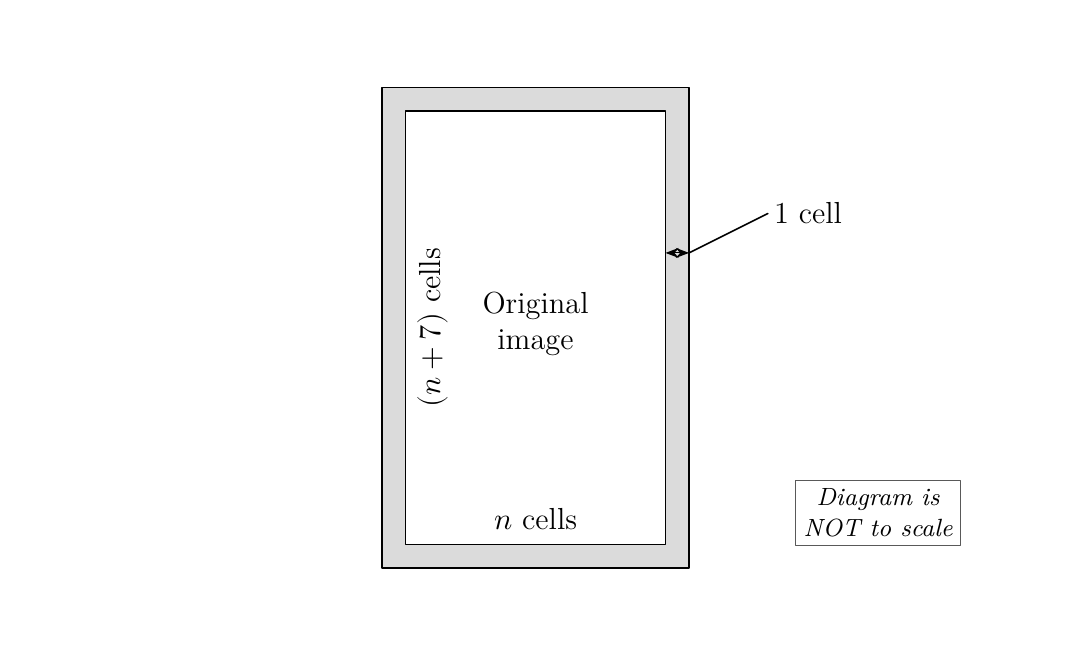
\begin{tikzpicture}
  \filldraw[fill=black!14] (4.5,.8) rectangle (8.4,6.9);
  \filldraw[fill=white] (4.8,1.1) rectangle (8.1,6.6);
  \node[align=center] at (6.45,3.9) {Original\\image};
  \node[above=3pt] at (6.45,1.1) {$n$ cells};
  \node[rotate=90] at (5.15,3.85) {$(n+7)$ cells};
  \draw[dimension] (8.1,4.8)--(8.4,4.8);
  \draw (8.4,4.8)--(9.4,5.3);
  \node[right] at (9.4,5.3) {1 cell};
  \NotToScale{(10.8,1.5)}
  \ExamBounds{130}{76.60714}
\end{tikzpicture}
\end{document}
